\documentclass[11pt, letterpaper]{article}
\usepackage[utf8]{inputenc}
\usepackage[english]{babel}
\usepackage[margin=1.5cm]{geometry}
\usepackage{titlesec}
\usepackage{tabu}
\usepackage{enumitem}
\usepackage{amssymb}
\usepackage{xcolor}
\usepackage{tikz}
\usetikzlibrary{shapes.geometric,shapes.misc,shapes.symbols,arrows.meta,graphs,fit,positioning,shadows}

\newlist{selectlist}{itemize}{2}
\setlist[selectlist]{label=$\square$,leftmargin=*,noitemsep,topsep=0pt}

\usepackage{lmodern}

\usepackage{hyperref}
\hypersetup{
    colorlinks=true,
    linkcolor=blue,
    filecolor=magenta,      
    urlcolor=blue,
}
 
\urlstyle{same}

% Set up the section label formatting
\titleformat{\section}[block]{\hspace{1em}\bfseries}{\thesection.}{0.5em}{} 
\titleformat{\subsection}[block]{\hspace{1em}}{\thesubsection}{0.5em}{}





%% 
%% Copyright 2007, 2008, 2009 Elsevier Ltd
%% 
%% This file is part of the 'Elsarticle Bundle'.
%% ---------------------------------------------
%% 
%% It may be distributed under the conditions of the LaTeX Project Public
%% License, either version 1.2 of this license or (at your option) any
%% later version.  The latest version of this license is in
%%    http://www.latex-project.org/lppl.txt
%% and version 1.2 or later is part of all distributions of LaTeX
%% version 1999/12/01 or later.
%% 
%% The list of all files belonging to the 'Elsarticle Bundle' is
%% given in the file `manifest.txt'.
%% 

%% Template article for Elsevier's document class `elsarticle'
%% with numbered style bibliographic references
%% SP 2008/03/01

%\documentclass[preprint,12pt, a4paper]{elsarticle}

%% Use the option review to obtain double line spacing
%% \documentclass[authoryear,preprint,review,12pt]{elsarticle}

%% For including figures, graphicx.sty has been loaded in
%% elsarticle.cls. If you prefer to use the old commands
%% please give \usepackage{epsfig}

%% The amssymb package provides various useful mathematical symbols
%\usepackage{amssymb}
%\usepackage{hyperref}
%% The amsthm package provides extended theorem environments
%% \usepackage{amsthm}

%% The lineno packages adds line numbers. Start line numbering with
%% \begin{linenumbers}, end it with \end{linenumbers}. Or switch it on
%% for the whole article with \linenumbers.
%\usepackage{lineno}

%\journal{Software Impacts}

\begin{document}
\noindent
\textbf{COPSolver: open source software for solving combinatorial optimization and other decision problems - library for solving the multi-product p-batch processing time maximization problem}
\vskip0.5cm
\noindent
\textbf{Tatiana Balbi Fraga, Federal University of Pernambuco, Avenida Marielle
Franco, Bairro Nova Caruaru, Caruaru, 55014-900, PE, Brazil, tatiana.balbi@ufpe.br}\\

\noindent
\textbf{Abstract}\\
COPSolver is an open source software originally developed to solve decision and/or optimization problems, especially from the combinatory optimization area. The first version of COPSolver has a application of Fraga's exact method for solving the multi-product p-batch processing time maximization problem. Such application can have significant impacts on software development for efficiently solving p-batch problems as well as contributing to better inventory control in some industries. Also it can be applied to conduct case studies, contributing to teaching and research. This paper address some important aspects of COPSolver and the next steps that will be implemented for it's applications development.
\vskip0.5cm

\noindent
\textbf{combinatorial optimization problem; exact method; p-batch problem; processing time maximization.}\\
\vskip0.5cm
\newpage
\noindent
\textbf{Code metadata}\\

%\begin{table}[!h]
\noindent
\begin{tabular}{|l|p{6.5cm}|p{9.5cm}|}
\hline
\textbf{Nr.} & \textbf{Code metadata description} & \textbf{Please fill in this column} \\
\hline
C1 & Current code version & COPSolver\_1.0-1 \\
\hline
C2 & Permanent link to code/repository used for this code version & $https://github.com/tbfraga/COPSolver/releases/tag$ $/v1.0\textrm{-}1$ \\
\hline
C3  & Permanent link to Reproducible Capsule & $https://codeocean.com/capsule/4837209$\\
\hline
C4 & Legal Code License   & Creative Commons Attribution-NonCommercial-NoDerivatives 4.0 International Public License \\
\hline
C5 & Code versioning system used & git \\
\hline
C6 & Software code languages, tools, and services used & c++, CodeBlocks, LINGO, Ubuntu 22.04.1, GitHub\\
\hline
C7 & Compilation requirements, operating environments \& dependencies & elementary OS (can be adapted to Ubuntu) \\
\hline
C8 & If available Link to developer documentation/manual & \underline{$http://tbfraga.github.io/COPSolver/documentation/$} \\
\hline
C9 & Support email for questions & tbfraga@proton.me\\
\hline
\end{tabular}\\
%\caption{Code metadata (mandatory)}
%\label{} 
%\end{table}
\vskip0.5cm
\noindent

\section{Motivation and significance}

A decision problem arises when we need to choose an option from a set of known options so that the chosen decision meets a set of pre-established constraints. This problem is configured as an optimization problem when the decision taken must, in addition to meeting the constraints, be the one that best contributes to the achievement of a given group of objectives.

Decision and/or optimization problems are frequent in industrial and organizational environments, as well as in our daily lives. Usually the resolution of these problems brings great benefits, such as improving the efficiency of industrial processes, reducing costs, increasing productivity, increasing the useful life of equipments, helping to make better choices, bringing better cost-effectiveness, improving customer satisfaction, etc.

Given the enormous variety of decision-making and/or optimization problems and the complexity of such problems, the literature brings numerous scientific materials that deal with the various problems and propose different solution methodologies for these problems. However, it is rare to find software that solves such problems. Usually such software is closed code, developed directly to solve very specific organizational problems, and the rights of use are kept by the developers and organizations involved in the software development project. Even when this does not occur, many pieces of software developed in research projects are simply not disclosed and end up being lost over time.

For this reasons I have developed COPSolver (Combinatorial Optimization Problems Solver), to make available to everyone cientific tools that can help improve the decision management process as well as improve the efficiency of various organizational processes.

\section{Software description}

COPSolver software was (and is being) developed by Dr. Tatiana Balbi Fraga with the purpose of solving several decision and optimization problems in the most efficient and robust way possible.

The first version of the software, COPSolver\_1.0-1, applies the exact solution method developed by Fraga et al. (2023) to solve the multi-product p-batch processing time maximization (MBPTM) problem. This problem arises in production process operations where a set of products are processed simultaneously on the same machine, but with production rates that can be different for each product. There is a production limit for each product and also for the products group, as well as a limit for the batch processing time. The problem consists of defining the maximum processing time of the multi-product batch respecting the known restrictions. The exact method of Fraga et al. (2023) is extremely efficient, proposing solutions very quickly and with low computational cost. 

COPSolver package also contains the MBPTM.lng file, which is a code written in LINGO language to solve the model proposed by Fraga et al. (2023) for the MBPTM problem. When run, COPSolver automatically generates a data.ldt file to be used with this LINGO code. However, the MBPTM.lng file can only be used through the LINGO software. More details about the LINGO software are available at https://www.lindo.com.

\subsection{Software architecture}

COPSolver is an open source software written in C++ language. Its architecture has been planned as follows: solver will be formed by a main.cpp file along with a library set (.h) and their respective source codes (.cpp). Each library will be developed to define and solve a single distinct type of problem. All libraries will contain two main structures called problem and solution, which will be used to define the parameters of the problem and the desired solution, respectively. Each library will also contain a class, called cop (for combinatorial optimization problems) or otherwise according to the nature of the problem addressed. Such class will basically contain functions for constructing/reading the problem, functions for solving the problem, and printing functions. Functions with similar purposes will be named with the same name using the functionalities of polymorphism. The libraries will be distinguished by a distinct namespace containing an acronym that identifies the problem addressed in the library itself. The definition of the problems instances can be done in three distinct ways: 1) through the data.txt file; 2) using solver predefined problems; and 3) generating a problem statically or randomly through pre-established functions of the solver. The config.txt file should be adjusted in order to: 1) inform the type of problem addressed; 2) select the method of defining the problem and the parameters that should be adjusted according to the chosen method; and 3) select the method for solving the problem. In the future, an extra library will be developed for automatic identification of the problem according to the definitions presented and for solution by the best method. For better suitability to the codeocean repository, the computational codes will be allocated within a folder named code, the files containing the input data (config.txt and data.txt) will be allocated within a folder named data, and the output files will be inserted into a folder named results. Also, files containing .h computational codes will be inserted inside a subfolder named lib while .cpp files (except main.cpp) will be inserted inside a subfolder named src. The lingo-language solvers developed for COPSolver validation will be available in specific subfolders within the folder named LINGOSolver.

\begin{figure}[h]
\begin{center}
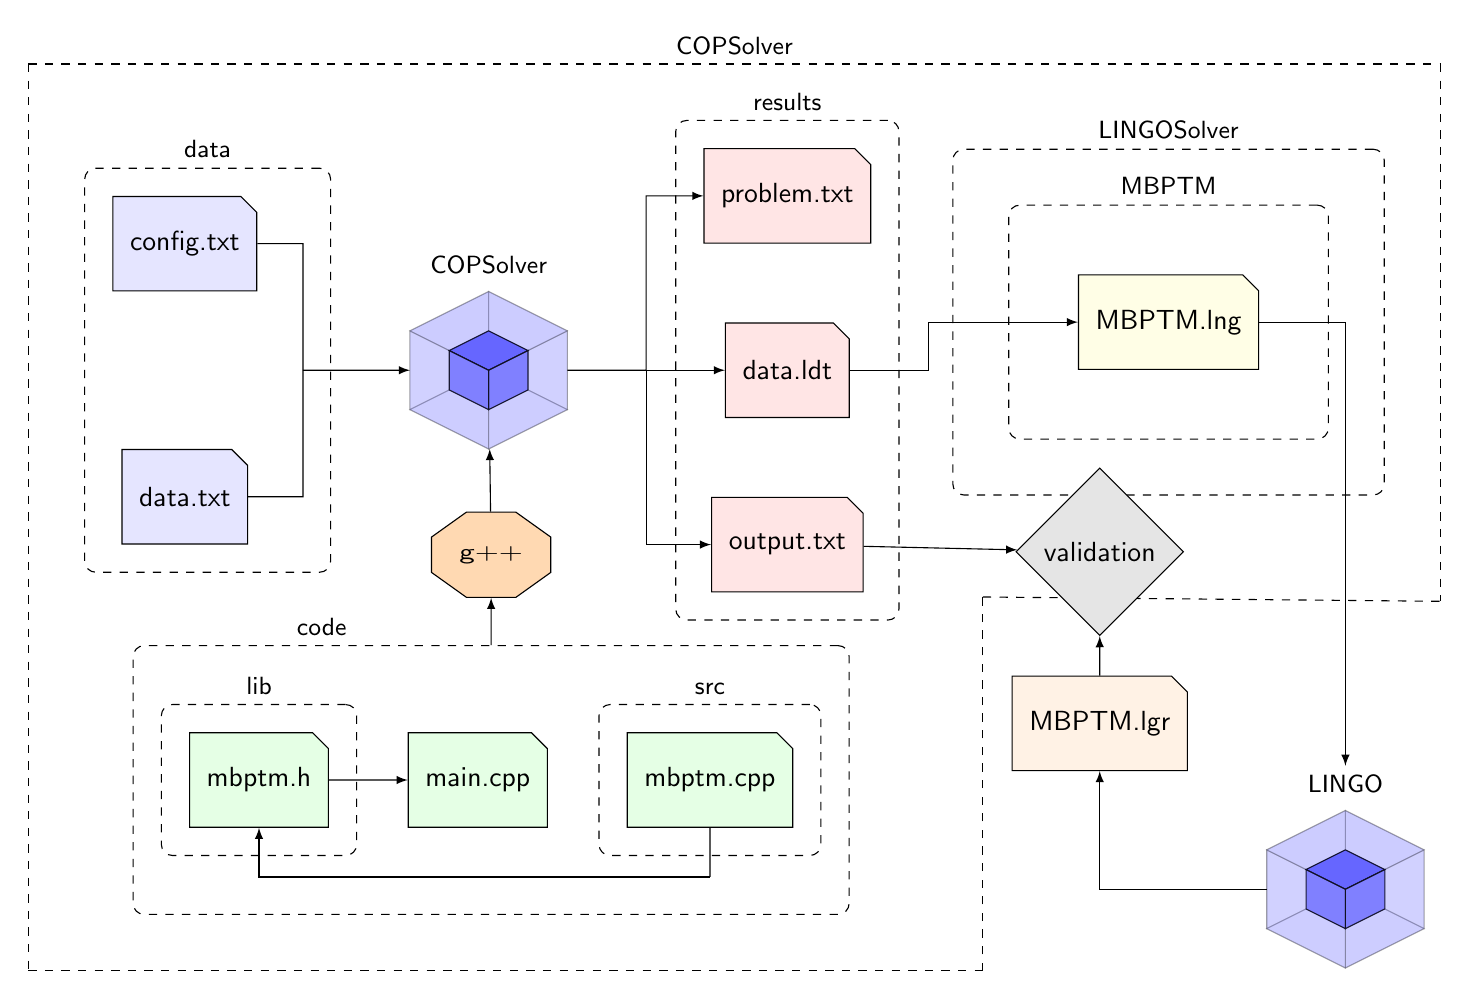
\begin{tikzpicture}[font=\sffamily,every label/.append style={font=\small\sffamily,align=center}]
\tikzset{doc/.style={chamfered rectangle, draw, chamfered rectangle corners=north east, fill=blue!10,draw,thin,minimum height=1.2cm,align=center},
pics/.cd,
pack/.style={code={%
\draw[fill=blue!50,opacity=0.2] (0,0) -- (0.5,-0.25) -- (0.5,0.25) -- (0,0.5) -- cycle;
\draw[fill=blue!50,opacity=0.2] (0,0) -- (-0.5,-0.25) -- (-0.5,0.25) -- (0,0.5) -- cycle;
\draw[fill=blue!60,opacity=0.2] (0,0) -- (-0.5,-0.25) -- (0,-0.5) -- (0.5,-0.25) -- cycle;
\draw[fill=blue!60] (0,0) -- (0.25,0.125) -- (0,0.25) -- (-0.25,0.125) -- cycle;
\draw[fill=blue!50] (0,0) -- (0.25,0.125) -- (0.25,-0.125) -- (0,-0.25) -- cycle;
\draw[fill=blue!50] (0,0) -- (-0.25,0.125) -- (-0.25,-0.125) -- (0,-0.25) -- cycle;
\draw[fill=blue!50,opacity=0.2] (0,-0.5) -- (0.5,-0.25) -- (0.5,0.25) -- (0,0) -- cycle;
 \draw[fill=blue!50,opacity=0.2] (0,-0.5) -- (-0.5,-0.25) -- (-0.5,0.25) -- (0,0) -- cycle;
\draw[fill=blue!60,opacity=0.2] (0,0.5) -- (-0.5,0.25) -- (0,0) -- (0.5,0.25) -- cycle;
}}}
\node[doc] (config) {config.txt};
\node[below=2cm of config, doc] (data) {data.txt};
\draw[-] (config) -- ++ (1.5,0) |- (data) coordinate[pos=0.25] (aux1);

\node[draw,dashed,rounded corners,fit=(config) (data) (aux1),inner sep=10pt,label={above:{data}}](fit1){};

\pic[right=2cm of fit1,local bounding box=code,scale=2] (COPSolver) {pack};
\node[above=1mm of code,font=\small\sffamily,align=center]{COPSolver};

\draw[-latex] (aux1) -- (code);

\node[right=2cm of code.east,doc,fill=red!10] (datalng) {data.ldt};
\node[above=1cm of datalng, doc, fill=red!10] (problem) {problem.txt};
\node[below=1cm of datalng, doc, fill=red!10] (output) {output.txt};
\node[draw,dashed,rounded corners,fit=(problem) (datalng) (output),inner sep=10pt,label={above:{results}}](fit2){};

\draw[-latex] (code) -- ++ (2,0) coordinate(aux2) |- (problem);
\draw[-latex] (aux2) |- (datalng);
\draw[-latex] (aux2) |- (output);

\node[below left =3.7cm and -0.65cm of code.south,doc,fill=green!10] (main) {main.cpp};
\node[left=1cm of main,doc,fill=green!10] (mbptmh) {mbptm.h};
\node[right=1cm of main,doc,fill=green!10] (mbptmcpp) {mbptm.cpp};

\node[draw,dashed,rounded corners,fit=(mbptmh),inner sep=10pt,label={above:{lib}}](fit3){};
\node[draw,dashed,rounded corners,fit=(mbptmcpp),inner sep=10pt,label={above:{src}}](fit4){};

\node[below=0.5cm of main] (aux2) {};
\node[above=0.5cm of main] (aux3) {};

\draw[-latex] (mbptmh) -- (main);

\node[below=0.5cm of mbptmcpp] (aux6) {};

\draw (mbptmcpp) -- (aux6.center);
\draw[-latex] (aux6.center) -| (mbptmh);

\node[draw,dashed,rounded corners,fit=(main) (fit3) (fit4) (aux2) (aux3),inner sep=10pt,label={above left:{code}}](fit5){};

\node[above=0.6cm of fit5, doc,regular polygon,regular polygon sides=8,fill=orange!30, scale=0.8, xscale=1.4] (compiler) {g++};

\draw[-latex] (fit5) -- (compiler);
\draw[-latex] (compiler) -- (code);

\node[above right=-0.5cm and 3cm of datalng,doc,fill=yellow!10] (lingocode) {MBPTM.lng};

\draw[-latex] (datalng.east) -- ++ (1,0) coordinate(aux6) |- (lingocode.west);

\node[draw,dashed,rounded corners,fit=(lingocode),inner sep=25pt,label={above:{MBPTM}}](fit6){};
\node[draw,dashed,rounded corners,fit=(fit6),inner sep=20pt,label={above:{LINGOSolver}}](fit7){};

\node[draw,dashed,rounded corners, white,fit= (fit1) (fit2) (fit5) (fit7),inner sep=20pt,label={above:{COPSolver}}](fit8){};

\draw[dashed](fit8.north west) -- (fit8.north east);
\draw[dashed](fit8.north west) -- (fit8.south west);

\node[right=12cm of fit8.south west] (aux3) {};

\draw[dashed](fit8.south west) -- (aux3.center);

\node[above=4.5cm of aux3] (aux4) {};

\draw[dashed](aux3.center) -- (aux4.center);

\node[below=6.7cm of fit8.north east] (aux5) {};

\draw[dashed](fit8.north east) -- (aux5.center);
\draw[dashed](aux4.center) -- (aux5.center);

\pic[below right=5cm and -0.5cm of fit7,local bounding box=lingo,scale=2] (LINGO) {pack};
\node[above=1mm of lingo,font=\small\sffamily,align=center](cap){LINGO};

\draw[-latex] (lingocode.east) -| (cap);

\node[above left=0.5cm and 1cm of lingo,doc,fill=orange!10] (outputlng) {MBPTM.lgr};

\node[above=0.5cm of outputlng, doc, shape=diamond, fill=black!10] (val) {validation};

\draw[-latex] (lingo.west) -| (outputlng.south);

\draw[-latex] (outputlng) -- (val);
\draw[-latex] (output) -- (val);

\end{tikzpicture}
\end{center}
\caption{Software architecture.}
\end{figure}

\section{Impacts}

Some industrial equipment process a set of jobs (batches) simultaneously. For production scheduling in these equipment, in addition to the sequencing and determination of the batches sizes, it is also necessary to define the set of batches that will be processed simultaneously in each time interval. These compound batches are called p-batch (parallel batching). Since most of p-batch problems are NP-Hard, many scientific works propose different local search heuristics for solving these problems (Fowler and Mönch, 2022). When applying some local search heuristics for solving a p-batch problem, it becomes necessary to determine the maximum p-batch processing time at each iteration. So, the method applied to solve this subproblem can have a strong impact on the computational cost of the local search algorithm proposed for solving p-batch problems. As reported earlier, COPSolver's library for solving the multi-product p-batch processing time maximization problem has an application of the Fraga's method to solve this subproblem, which has very low computational cost. Therefore, this library can be used to implement local search heuristics-based algorithms developed for solving p-batch problems, generating a high impact on the efficiency of these algorithms. An article has been submitted for publication, which present the exact method proposed for solving multi-product p-batch processing time maximization problems as well as an extensive study on the computational efficiency of the COPSolver\_1.0-1 (Fraga \emph{et al.}, 2023). In order to make this software available to the rest of the world, all the necessary files that is required to compile and run the software successfully have been published to the codeocean project (Fraga, 2023).

It is important to note that the determination of the maximum processing time of multi-product p-batches itself is extremely important for some industries, as it is directly related to inventory management as well as to the correct fulfillment of demand. Therefore, COPSolver\_1.0-1 can serve as an important tool for inventory control, reducing costs and improving demand compliance. As future works, we will be applying COPSolver to assist in planning and scheduling the production of extruders, in companies of the plastic bag production sector. With this we hope to improve inventory management, increasing the competitive potential of these companies. These works will be case studies, conducted to assist in teaching and research, so it can also generate an important impact in these aspects.


\section{Next steps}

Professor Fraga, author of this paper, and, more generally, her research group GAMOS (Group of Analysis, Modeling and Optimization of Systems), have developed many works focused on the identification, modeling and solution/optimization of real problems in industrial/organizational environments. Therefore, the development of COPSolver will be done in conjunction with the development of these works. Our intention is that the software can, in the near future, cover a wide range of methodologies to solve real problems and standard problems found in the literature. Later we intend to develop a pattern identification method to recognize problems patterns and solve different problems automatically. In the future, we will also be developing extension projects to train micro and small companies to use COPSolver. We hope that COPSolver can help to improve several processes and, in particular, the productive and administrative processes of micro and small companies, offering them a tool to improve their competitive potential.

\vskip0.3cm
\noindent
\textbf{Declaration of competing interest}\\
The authors declare that they have no known competing financial interests or personal relationships that could have appeared to influence the work reported in this paper.

\vskip0.3cm
\noindent
\textbf{Acknowledgements}\\
Huge thanks to the teams responsible for developing elementary OS, as well as google translator, duckduckgo, gummi, CodeBlocks, LINGO, git, GitHub, gcc, and TeXLive libraries. Without the availability of these tools, COPSolver could never have been developed. I am also very grateful to my co-workers Regilda da Costa e Silva Menêzes and Marcos Luiz Henrique for their constant support to the projects I develop and to my dear advisees Aldênia Karla Barrêto Candido, Lays Cristiane Cavalcante de Alcântara Aguiar, Edwedja de Lima Silva and Ítalo Ruan Barbosa de Aquino, among others, for having participated so enthusiastically in the projects that gave rise to this software, in particular for having made the effort to describe real processes in such detail. I would also like to thank the company in the plastic bag sector and other companies that made the studies possible as well as the identification of the new optimization problem addressed in COPSolver\_1.0-1. \\

\noindent
\textbf{References}\\

Fraga, T.B., Aquino, Í.R.B. and Menêzes, R.C.S. (2023). Exact method for solving the multi-product p-batch processing time maximization problem. Manuscript submitted for publication.  \\

Fraga, T.B. (2023). COPSolver: open source software for solving combinatorial optimization and other decision problems - library for solving the multi-product batch processing time maximization problem. Published Version 1.0. codeocean. Available at: https://codeocean.com/capsule/4837209/tree/v1.  \\

Fowler, J.W. and Mönch, L. (2022). A survey of scheduling with parallel batch (p-batch) processing. European Journal of Operational Research, v. 298, pp. 1–24. \\


\vskip 1.5cm

\end{document}
%\endinput
%%
%% End of file `SoftwareX_article_template.tex'.
